% Diese Zeile bitte -nicht- aendern.
\documentclass[course=erap]{aspdoc}

\usepackage{algorithm}
\usepackage{algpseudocode}
\usepackage{amsmath}
\usepackage{subcaption}
\usepackage{tikz}
\usepackage{array}
\usepackage{graphicx}
\usepackage{tabularx}
\usepackage{pgfplots}
\pgfplotsset{compat=1.17}
\pgfplotsset{compat=newest}
%%%%%%%%%%%%%%%%%%%%%%%%%%%%%%%%%
%% TODO: Ersetzen Sie in den folgenden Zeilen die entsprechenden -Texte-
%% mit den richtigen Werten.
\newcommand{\theGroup}{158} % Beispiel: 158
\newcommand{\theNumber}{A206} % Beispiel: A206
\author{Lukas Li \and Yassine Hmidi \and Constantin Carste}
\date{Wintersemester 2023/24} % Beispiel: Wintersemester 2023/24
%%%%%%%%%%%%%%%%%%%%%%%%%%%%%%%%%

% Diese Zeile bitte -nicht- aendern.
\title{Gruppe \theGroup{} -- Abgabe zu Aufgabe \theNumber}

\begin{document}
\maketitle

\section{Einleitung}
Im Bereich der digitalen Bildverarbeitung führt die Schnittstelle zwischen mathematischen Prinzipien und realer Anwendung zu vielen innovativen Algorithmen, die den jetzigen Stand der Technik verbessert. Dieses Projekt befasst sich mit der Bildmanipulation und spezialisiert sich insbesondere auf der Umwandlung von Farbbildern in Graustufen und eine anschließende Skalierung durch bilineare Interpolation. Dazu werden theoretische Erkenntnisse aus der Mathematik genutzt, um einen praktischen C-Algorithmus zu entwickeln.\\
Jedes Farbbild besteht aus Pixeln, die durch ihre Position $(x, y)$ eindeutig identifiziert sind und durch ihren Farbvektor (R, G, B) definiert werden. Die erste Herausforderung besteht darin, diese Farbpixel in Graustufen umzuwandeln. Dabei wird ein gewichteter Durchschnitt der Einträge des Farbvektors mit geeigneten Koeffizienten $a$, $b$ und $c$ berechnet. Bei der Berechnung der Grauwerte wird Rücksicht auf die Wahrnehmung des menschlichen visuellen Systems (HVS) genommen, damit das entstandene Graustufenbild besonders ansprechend für die menschlichen Augen ist. Anschließend wird die bilineare Interpolation angewendet, um das Bild passend zu skalieren.\\\\
Die theoretische Grundlage dieses Projekts basiert auf dem Verständnis des 24bpp PPM-Bildformats, welches als Eingabe erwartet wird, sowie auf den mathematischen Berechnungen der Graustufenkonvertierung und der bilinearen Interpolation.\\
Auf der praktischen Seite erstreckt sich die Aufgabe über die Umsetzung der theoretischen Erkenntnisse in der Programmiersprache C. Die Implementierung des Algorithmus umfasst ebenso ein Rahmenprogramm, das PPM-Dateien und weitere optionale Parameter über die Kommandozeile entgegennimmt und das Ergebnis der Berechnung als ein PGM-Bild abspeichert. Durch die I/O-Funktionen des Rahmenprogramms wird eine praktische Einbindung des Resultats in weitere Projekte und das Anpassen des Algorithmus an verschiedene Szenarien ermöglicht.\\
Während der Ausarbeitung des Projektes wird insbesondere der Fokus auf die Optimierung gelegt – theoretisch durch algorithmische Optimierung und praktisch durch Parallelisierung und SIMD.

\begin{figure}[ht]
    \centering
    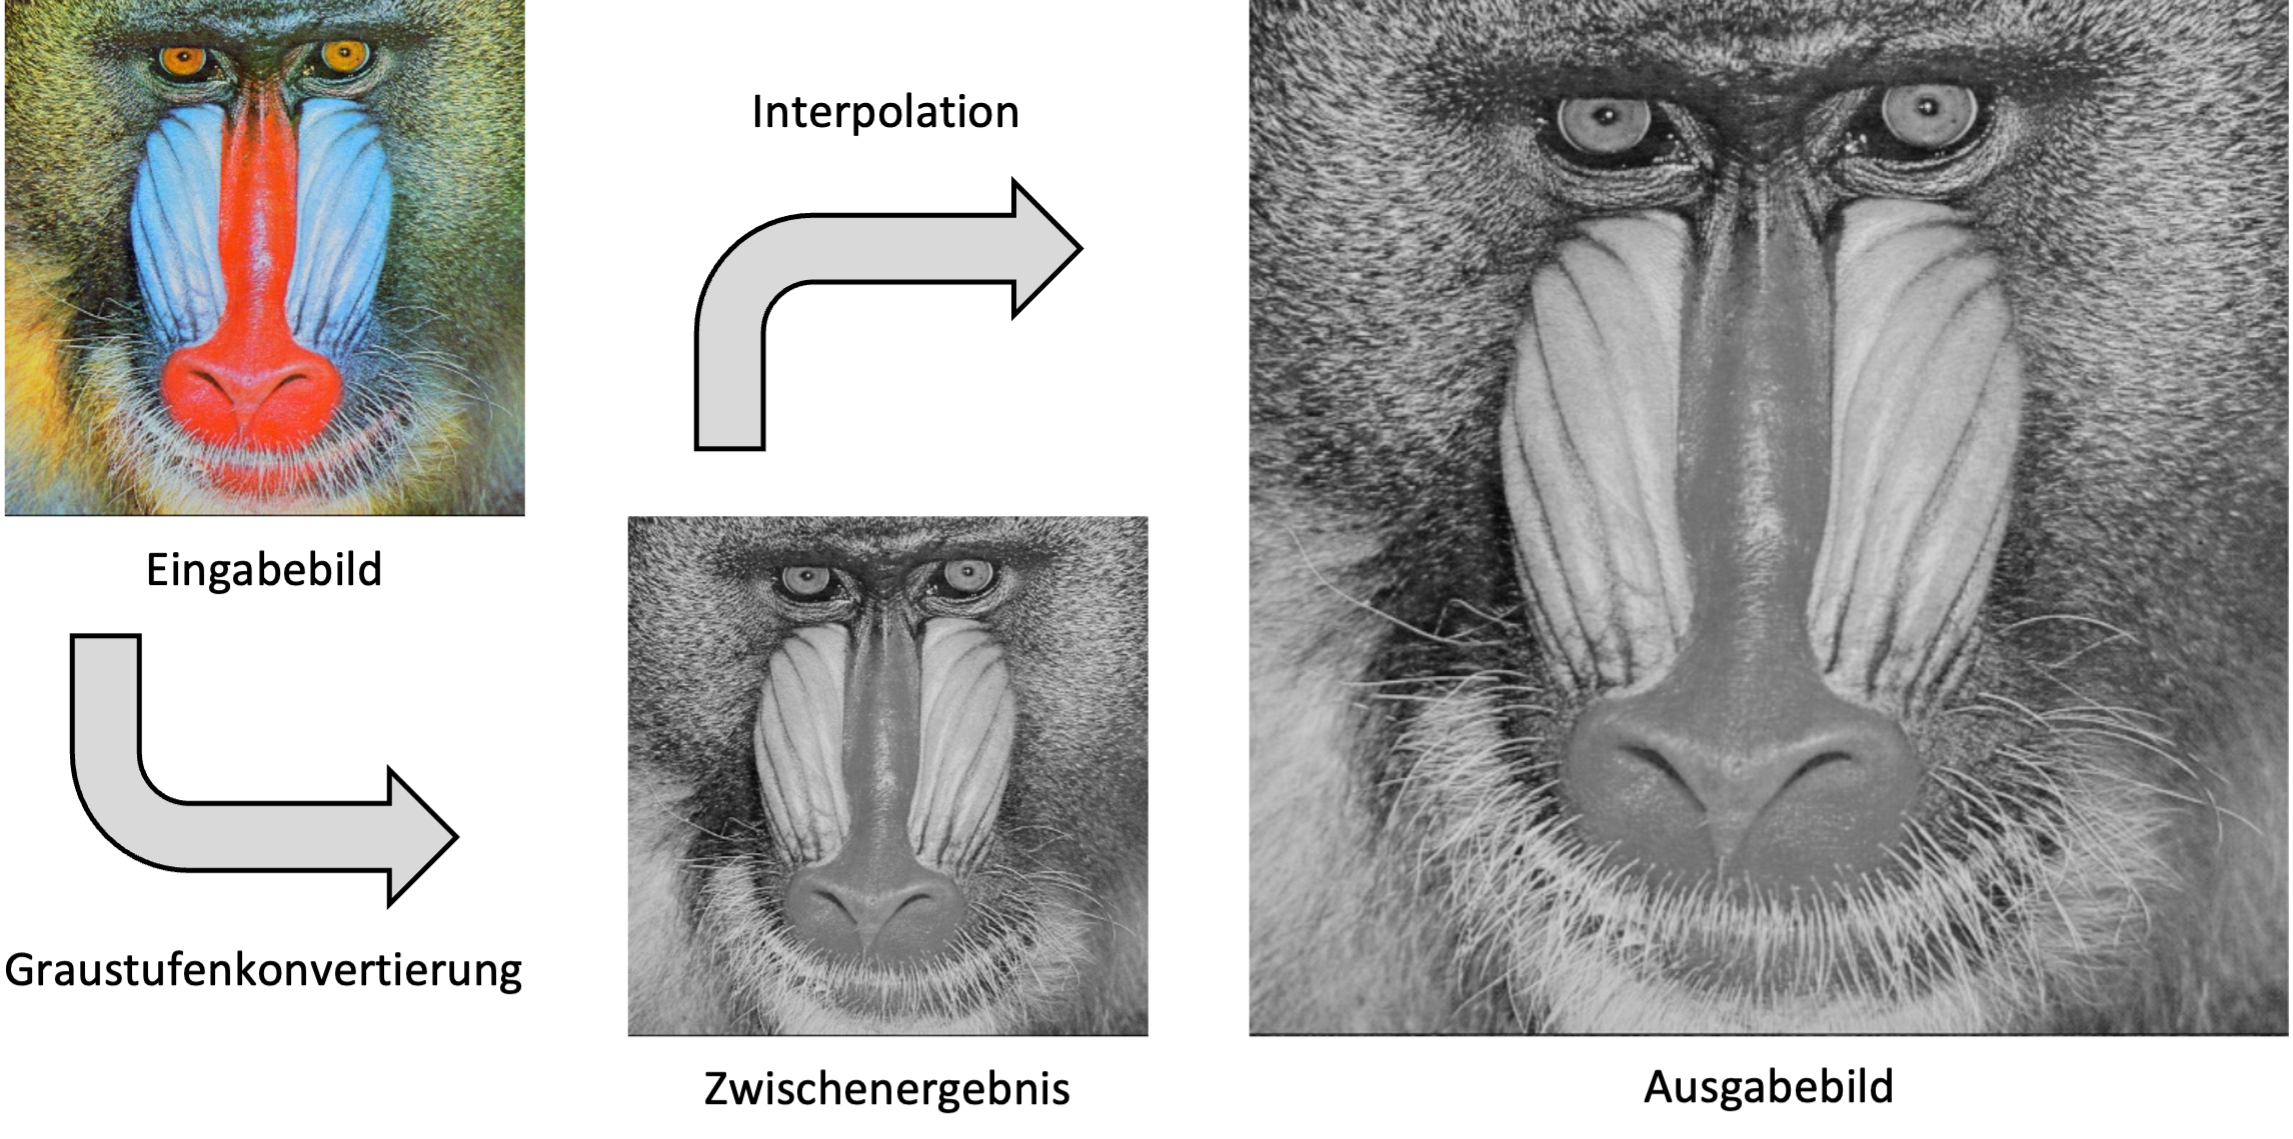
\includegraphics[scale=0.8]{assets/verlauf.png}
    \caption{Verlauf der Eingabe zur fertigen Ausgabe}
    \label{fig:verlauf}
\end{figure}

\section{Lösungsansatz}
Das Programm muss die Nutzereingaben korrekt erkennen und bei fehlerhaften Eingaben sinnvolle Alternativwerte verwenden.\\
Die eigentliche Konvertierung wird in drei Teilsektionen aufgeteilt. Die Graustufenkonvertierung konvertiert die PPM-Eingabe zu einem PGM-Bild, wobei die dafür vorgesehene Rundung nicht vorgenommen wird, die Interpolation skaliert das Grayscaling-Resultat mit dem vom Benutzer angegebenen Faktor und gibt dieses aus.

\subsection{Netpbm-Format}
Das Netpbm-Format enthält neben ppm auch das pgm-Bildformat. Dabei wird die Ausgabe ein P5 PGM sein. Die Entscheidung für ein PGM-Bild als Ausgabedatei lässt sich damit begründen, dass PGM für Graustufenbilder optimiert ist und nur ein Drittel der Speicher verbraucht wie das gleiche Bild als PPM abzuspeichern. Dabei verwenden PGM und PPM den gleichen Header (bei PPM P6 und bei PGM P5 als magischer Nummer). Anschließend speichert ein PPM-Bild für jeden Pixel die drei Farbkanäle Rot, Grün und Blau ab. Da beim Graustufenbild für alle drei Kanäle den gleichen Wert verwendet wird, trifft PPM-Bild die Vereinfachung, für jeden Pixel nur einen Wert abzuspeichern und braucht somit viel weniger Speicher als PPM.

\subsection{Rahmenprogramm}
Im Zuge der Implementierung war es nötig, ein Rahmenprogramm für die einfache Benutzererfahrung zu erstellen. Dabei wurde besonders viel Rücksicht auf die Benutzerfreundlichkeit genommen. Bis auf das Eingabebild sind alle Parameter optional und müssen nicht gesetzt werden. Dabei wird als Eingabebild ein 24bpp P6 ppm Bild erwartet (das heißt, für jeden Farbkanal Rot, Grün und Blau darf nicht mehr als ein Byte verwendet werden, außerdem darf die Luminanz nicht gesetzt werden). Falls die Parameter nicht gesetzt oder falsch sind wie beispielsweise ein ungültiger Dateiname für Ausgabedateien, wird nach einer kurzen Warnung auf der Konsole auf Standardwerte zurückgegriffen. Bei fehlenden Parameter für das Eingabebild oder ungültiges Eingabebild wie falsches Bildformat wird das Programm mit einer Fehlermeldung terminiert. Die Funktion $interpolate($...$)$ speichert das Graustufenbild in $tmp$ und das interpolierte Bild in result ab. Anschließend schreibt das Rahmenprogramm das Bild als ein P5 PGM-Bild unter den gesetzten Parameter in den Speicher.

\subsection{Graustufenkonvertierung}
Die Graustufenkonvertierung sieht vor, das vom Benuter angegebene PPM Bild in ein PGM-Bild umzuwandeln. Ein PPM-Bild hat für jeden Pixel drei Werte gegeben (R, G, B), ein PGM-Bild nur einen, da das Bild für alle drei Kanäle die gleichen Werte verwendet. Die R, G und B Werte müssen also mit Koeffizienten (a, b und c) zu einem einzelnen Wert $D$ gewichtet werden.
 \begin{align}
    D_{neu} {=} \frac{a \cdot R + b \cdot G + c \cdot B}{a + b + c}
\end{align}
Um jede Konvertierung zu optimieren, muss $a + b + c = 1$ gegeben sein, da dadurch eine Division für jeden Pixel gespart werden kann. Die Koeffizienten werden also vor der Konvertierung miteinander skaliert.
 \begin{align}
    D_{neu} \underset{a + b + c = 1}{=} a \cdot R + b \cdot G + c \cdot B
\end{align}

\subsubsection{Koeffizientenwahl}
Die Standard-Koeffizienten $a = 0.299 (\approx \frac{2}{7}), b = 0.587 (\approx \frac{4}{7})$ und $c = 0.144 ( \approx \frac{1}{7})$ sind aufgrund der Annahme, dass das menschliche Auge Grün stärker als Rot und Rot stärker als Blau wahrnimmt, getroffen worden. Damit ergibt sich ein dem menschlichen Wahrnehmungssystem besonders ansprechende Graustufenbild. Diese Koeffizienten addieren somit standardgemäß bereits auf $1$ auf, wodurch die Konvertierung übersprungen werden kann. 


\subsubsection{Naive Konvertierung}
Die naive Konvertierung sieht vor, jeden Pixel einzeln zu berechnen und in einem Float-Array abzuspeichern. Dadurch wird mit verschiedenen Graustufenintensitäten die Helligkeitsstufen im ursprünglichen Farbbild sichergestellt, wodurch das resultierende Bild mehr Details erhält.

\subsubsection{Konvertierung mit Tabellen}
Für diesen Konvertierungsansatz werden vorberechnete Tabellen verwendet, die jedes mögliche Ergebnis der Multiplikation von 0 bis 255 (bzw. dem maximalen Farbwert) mit den entsprechenden Koeffizienten enthalten. Aufgrund der Größenlimitierung durch den Farbwert könnte ihre Zuweisung lokal im Stack erfolgen. Die Idee besteht darin, dass wir die Berechnung des Zwischenmultiplikationswertes für redundante Farbkanäle zu vermeiden. Statt der Multiplikation werden die Werte in der Tabelle nachgeschlagen und zum endgültigen $D_{neu}$ addiert.

\subsubsection{Konvertierung mit SIMD}
In unserer Implementierung wird SIMD  eingesetzt, um vier Pixel gleichzeitig zu verarbeiten und so die Effizienz gegenüber einer sequenziellen Bearbeitung zu steigern. Da SIMD ausgerichtete Daten voraussetzt, werden die letzten Pixel individuell und nicht mit SIMD verarbeitet.\\

\begin{algorithm}
\caption{Grayscale conversion using SIMD}
\small % Makes the font smaller
\begin{algorithmic}[1]
    \State $coef \gets ((a, a, a, a), (b, b, b, b), (c, c, c, c))$ \Comment{Init coeffs}
    \State $end \gets h \cdot w \cdot 3 - (h \cdot w \cdot 3 \mod 12)$
    \For{$i \gets 0$ \textbf{to} $end$ \textbf{step} $12$} \Comment{Aligned data}
        \State $vecR \gets (R_{1}, R_{2}, R_{3}, R_{4})$
        \State $vecG \gets (G_{1}, G_{3}, G_{3}, G_{4})$
        \State $vecB \gets (B_{1}, B_{3}, B_{3}, B_{4})$
        \State $Ra, Gb, Bc \gets vecR \cdot coef[0], vecG \cdot coef[1], vecB \cdot coef[2]$
        \State $D \gets Ra + Gb + Bc$ \Comment{Grayscale}
        \State $res[i/3] \gets \text{Round}(D)$ \Comment{Rounding}
    \EndFor
    \For{$i \gets end$ \textbf{to} $h \cdot w \cdot 3$ \textbf{step} $3$} \Comment{Remaining}
        \State $res[i/3] \gets \text{round}(a \cdot img[i] + b \cdot img[i+1] + c \cdot img[i+2])$
    \EndFor
\end{algorithmic}
\end{algorithm}


\subsection{Interpolation}
Das Ziel der Interpolation ist es, eine Bildskalierung durchzuführen, also ein Bild so zu vergrößern, dass das menschliche Auge möglichst wenig Unschärfe erkennen kann. Hierfür werden einzelne Pixel mit einem Skalierungsfaktor $k$ voneinander verschoben, wodurch Löcher von $k-1$ Pixeln im neu generierten Bild entstehen, welche mit Zwischenwerten aufgefüllt werden. Zwei zuvor aneinandergrenzende Pixel mit $k = 2$, einer schwarz, der andere weiß, sollten also in einem grauen Pixel resultieren. Da die Verschiebung in der Höhe sowie Breite durchgeführt wird entsteht pro Pixel ein neues Quadrat der Größe $k \cdot k$, mit dem ursprünglichen Pixel in der oberen linken Ecke. Durch Ausweitung des Quadrats auf $(k+1) \cdot (k+1)$ erhält man
ein Quadrat, dessen Eckpunkte bekannt sind. Anhand der bekannten Pixel kann man die restlichen Pixel mit der folgenden Formel berechnen und befüllen. Für die mathematische Berechnung werden die Pixel in einem Koordinatensystem mit $x, y \in [0, k]$ angegeben. Also haben die vier originalen Eck-Pixel folgende Koordinaten: $(0, 0), (0, k), (k, 0)$ und $(k, k)$. Für die unbekannten zu interpolierenden Pixel an $(x, y)$ gilt dann die Formel
 \begin{align}
    Q_{neu} {=}  \frac{1}{(k)^2} \cdot
    \begin{pmatrix} k-y & y \end{pmatrix} \cdot
    \begin{pmatrix} Q_{(0,0)} & Q_{(0,k)} \\ Q_{(k,0)} & Q_{(k,k)} \end{pmatrix}
    \cdot
     \begin{pmatrix} k-x \\ x \end{pmatrix} 
\end{align}

 
mit $(x, y)$ als Koordinaten des zu berechnenden Pixels. Diese Funktion funktioniert für fast alle Quadrate, mit Ausnahme der rechten und unteren Randpixel, da diese keine Nachbar-Pixel haben, auf die das Quadrat ausgeweitet werden kann. Um die Interpolation weiter durchzuführen müssen also sinnvolle Alternativwerte gefunden werden.

\subsection{Interpolation der Randpunkte}
Bei der Interpolation der rechten sowie unteren Randpixel fehlen jeweils zwei bis drei der vier benötigten Eckpunkte (letzteres nur in der unteren rechten Ecke). Für diese Interpolation müssen also Alternativwerte gesucht werden.\\
Zum Verständnis sehen wir das Bild als Zylinder an. Dadurch berühren sich zwei Kanten, als Beispiel die linke und rechte Kante, und löst das Problem der unbekannten Eckpunkte für eine Kante auf. Im Klartext füllt man somit die unbekannten Eckpunkte mit den ersten Eckpunkten der aktuell bearbeitenden Reihe / Spalte. Dieser Ansatz würde jedoch beispielsweise bei einem Verlaufsbild von schwarz nach weiß zu einer ungewollten rechten Kante führen. Die meisten Bilder, haben jedoch einen gleichfarbigen Farbverlauf von links nach rechts (wie beispielsweise der Horizont eines Portraits), der unwahrscheinliche Fall eines Verlaufsbildes kann also in Kauf genommen werden.


\subsection{Interpolationsansätze}

\subsubsection{Naiver Interpolationsansatz}
In unserem ersten Interpolationsansatz iterieren wir über jedes Pixel des skalierten Bildes. Dabei werden Zwischenwerte, die für verschiedene x-Indizes bei gleichem y-Index gleich bleiben, im Voraus berechnet. Wir ermitteln die benötigten Pixelwerte aus dem Eingabebild in Graustufen, indem wir die entsprechenden Indizes berechnen. Anschließend führen wir die Interpolationsberechnung durch, konvertieren das Ergebnis und speichern es als $uint8\_t$-Wert im Ausgabebild. Dieses Format entspricht dem PGM-Format unseres Ausgabebildes.

\subsubsection{Algorithmisch optimierter Interpolationsansatz}
Der optimierte Interpolationsansatz bearbeitet das neue Bild in Sektoren - also in Quadraten der Größe $k \cdot k$, statt $(k+1) \cdot (k+1)$, da das in einer doppelten Berechnung der unteren und rechten Kante resultieren würde. Dabei sind immer drei der bekannten Randpunkte außerhalb des eigentlichen Quadrates, mit dem oberen linken Randpunkt als bekannter Pixel. Für jedes Quadrat werden die Eckpunkte aus dem PGM Bild ausgelesen und in Variablen abgespeichert, dass nicht jeder neue Pixel erneut auf die vier Pixel zugreifen muss. Daraufhin wird die Funktion für jeden Pixel ausgeführt - der resultierende Float wird gerundet und an korrekter Stelle im neuen Bild abgespeichert. Der uns bereits bekannte obere linke Pixel wird nicht berechnet sondern direkt eingesetzt. Falls der Skalierungsfaktor Eins entspricht, muss dieser Ansatz nicht ausgeführt werden beziehungsweise kann zu Beginn terminiert werden, da sich das Bild nicht verändert.

\subsubsection{Algorithmisch weiter optimierter Interpolationsansatz}
Der weiter-optimierte Interpolationsansatz basiert ebenfalls auf Sektoren. Die Idee hierbei ist, dass in horizontaler Richtung folgende Funktion genutzt werden kann, um die Werte zu berechnen. In der folgenden Funktion sei $k =$ Skalierungsfaktor, $x =$ Wert im Quadrat
\begin{align}
    Q_{x} {=} Q_{0} \cdot \frac{k-x}{k} + Q_{k} \cdot \frac{x}{k}
\end{align}
Dieser Ansatz wird auf die vertikale Richtung weitergeführt, wobei die entsprechenden $Q_{0}$ und $Q_{k}$ Werte berechnet werden müssen, da sie im neuen Bild bereits gerundet wurden. Die Berechnung der Werte unterscheidet sich dadurch von dem zweiten Ansatz eigentlich nur in der Reihenfolge.

\subsubsection{Interpolation mit SIMD}
Die Idee hier ist, dass wir das eingegebene Graustufenbild durchiteriert wird und die Tatsache ausgenutzt wird, dass jeder Pixel für einen Sektor als $Q_{0,0}$ interpretiert wird. Deshalb werden vier $Q_{0,0}$-Werte, die 4 aufeinanderfolgenden Sektoren entsprechen geladen. Das Gleiche gilt für die $Q_{s,0}$, wobei jetzt jede Zeile jeweils bei $x=1$ beginnt. Das gleiche Konzept gilt für $c$ und $d$, ausgenommen der ersten Linie. Die letzte Zeile und letzte Spalte, die zu den nicht ausgerichteten Daten hinzugefügt wurden, müssen einzeln behandelt werden.
\begin{algorithm}
\caption{SIMD-Interpolation Implementierung}\label{alg:simd_interpolation}
\begin{algorithmic}[1]
\State $breiteNeu \gets breite \times faktor$
\State $invFaktor \gets 1 / faktor$
\State Vorbereiten der Zwischenwerte außerhalb der Schleifen
\For {$y \gets 0$ \textbf{to} $hoehe - 2$}
    \For {$x \gets 0$ \textbf{to} $(breite - 1) - ((breite - 1) \% 4)$}
        \State $Q00 \gets$ Lade 4 aufeinanderfolgende Pixel
        \State $Qs0 \gets$ Lade 4 aufeinanderfolgende Pixel startend von $x + 1$ 
        \State $Q0s \gets$ Lade 4 Pixel von  Zeile
        \State $Qss \gets$ Lade 4 diagonalen Pixel startend von $x + 1$ 
        \For {$i \gets 0$ \textbf{to} $faktor - 1$}
            \For {$j \gets 0$ \textbf{to} $faktor - 1$}
                \State $a, b, c, d \gets$ Lade Zwischenwerte mit Shuffle
                
                \State $interpolated \gets Q00*a + Qs0*b + Q0s*c + Qss*d$                 
                \State Speichere gerundet und konvertierte interpolierte Werte
            \EndFor
        \EndFor
    \EndFor
    
\EndFor
\State Verarbeite Randpunkte mit nicht-SIMD-Prozess
\end{algorithmic}
\end{algorithm}

% TODO: Je nach Aufgabenstellung einen der Begriffe wählen
\section{Genauigkeit}
\subsection{Rechnen mit Floats}
Im allgemeinen wird bei der Graustufenkonvertierung sowie Interpolation mit Floats gearbeitet. Floats sind auf 32 Bit begrenzt und für ihre Ungenauigkeit bei der Multiplikation bekannt. Im Falle der Koeffizienten für die Graustufenkonvertierung können die Endresultate für die Optimierung $a + b + c = 1$ meistens nicht perfekt in Floats gespeichert werden. Als Alternative könnte man auf Doubles zurückgreifen, was aber einen Eingriff in den SIMD-Prozess aufgrund größerer Datenstrukturen ineffizient machen würde.

%\subsection{Graustufenkonvertierung zu Interpolation}
%Durch die normale Konvertierung zu einem PGM-Bild und #darauffolgender Interpolation würden die PGM-Werte gerundet %weiterverarbeitet werden. Stattdessen gibt die #Graustufenkonvertierung das Bild in Floats aus, wodurch die %%Interpolation genauere Werte zur Berechnung nutzen kann.

\subsection{Graustufenkonvertierung}
Bei der Entwicklung der Methoden zur Graustufenkonvertierung war es wichtig, eine einheitliche Rundungsstrategie zu verfolgen, um Konsistenz über alle Implementierungen hinweg zu gewährleisten. Bei der Anwendung der Lookup-Tabellen und der naiven Interpolationsmethode wurde dies beachtet.\\
Im Fall der SIMD-Implementierung musste aufgrund der fehlenden direkten Entsprechung einer exakten Rundungsmethode für einzelne Fließkommazahlen ein alternativer Ansatz gewählt werden. Hierbei wurde auf jeden Wert $0.5$ addiert und die Fließkommazahl durch $\_mm\_floor\_ps$ abgerundet. Diese Vorgehensweise kann im Vergleich zu anderen Methoden leicht langsamer sein, sichert jedoch eine exakte Rundung und garantiert, dass alle Konvertierungen unabhängig von der Eingabe konsistente und präzise Resultate liefern. Obwohl diese Methode möglicherweise nicht die schnellste ist, wurde sie gewählt, um die Genauigkeit zu maximieren und zu gewährleisten, dass die Ergebnisse exakt den mathematischen Erwartungen entsprechen.

\subsection{Interpolationsrundungen}
Die von der Interpolation berechneten neuen Pixel sind in den meisten Fällen Werte mit Nachkommastellen (Beispiel: $k = 2$ mit $P_{0,0} = 10$, $P_{1,0} = 11$ ergibt $Q_{0,0} = 10$, $P_{1,0} = 10.5$, $P_{2,0} = 11$, $...$). Der resultierende Wert muss also gerundet werden. Im Falle eines maximalen Farbwertes von $255$ kann diese Rundung eher vernachlässigt werden, würde aber bei niedrigen maximalen Farbwerten theoretisch Probleme bereiten. Daher wurde die in der Graustufenkonvertierung erwähnte Rundung via 0.5 verwendet, um bei allen Implementationen die gleichen Werte zu erzielen, bevor die Resultate in einem $uint\_8$ abgespeichert werden.

\subsection{Genauigkeit-Test}
\subsubsection{bei steigenden Anzahl von Pixeln:}
Die Genauigkeit wurde über ein breites Spektrum an Bildgrößen hinweg getestet, mit einem besonderen Fokus auf den Skalierungsfaktor 2. In jedem Fall, von kleinsten Bildern bis hin zu solchen mit 16 Millionen Pixeln, waren die Resultate identisch. Dies zeigt die Zuverlässigkeit der Implementierungen und die Effektivität der Rundungsmethoden, insbesondere der strategischen Addition von $0.5$ vor der Abrundung in der SIMD-Implementierung.\\
Die Algorithmen demonstrieren eine hohe Präzision und Konsistenz, was ihre Anwendbarkeit in der Praxis bestätigt.\\


\subsubsection{bei steigenden Skalierungsfaktoren:}

\begin{table}[ht]
\centering
\begin{tabular}{|c|c|c|c|c|c|c|}
\hline
k & \# Pixeln & v1 vs v2 & ER v1 vs v2 (\%) & v1 vs v3 & ER v1 vs v3 (\%)  \\ 
\hline
6 & 9437184 & 75751 & 0.803 & 51477 & 0.545  \\
10 & 26214400 & 36819 & 0.140 & 34006 & 0.130  \\
12 & 37748736 & 150131 & 0.398 & 103552 & 0.274  \\
14 & 51380224 & 61126 & 0.119 & 40514 & 0.079  \\
\hline
\end{tabular}
\caption{Vergleich der Implementierungen und Fehlerquote.}
\label{tab:comparison}
\end{table}

Es gibt bis zu einem Skalierungsfaktor von 5 keine Unterschiede in den Pixelwerten zwischen den drei Implementierungsmethoden bestehen. Ab einem Skalierungsfaktor von 6 treten geringfügige Differenzen auf, die jedoch nur eine Abweichung von 1 pro Pixel betragen. Diese minimale Diskrepanz ist vernachlässigbar und führt zu keinen sichtbaren Unterschieden im resultierenden Bild.

Die Ursache für die aufgetretenen Unterschiede liegt in der Verwendung von Fließkommazahlen und den damit verbundenen Rundungen sowie in den unterschiedlichen Berechnungsschritten der Methoden. s ist wichtig zu betonen, dass diese Abweichungen zwar aus technischer Sicht vorhanden sind, sie jedoch keinen Einfluss auf die praktische Anwendung der Bildbearbeitung haben. Die visuelle Qualität der Bilder bleibt unbeeinträchtigt, was die Effektivität und Zuverlässigkeit der untersuchten Implementierungen unterstreicht. Die Ergebnisse bestätigen daher unsere theoretische Annahme, dass solche Abweichungen im Rahmen der Bildverarbeitung akzeptabel sind, insbesondere wenn sie unterhalb der Wahrnehmungsschwelle des menschlichen Auges liegen.

\section{Performanzanalyse}
\subsection{Theorethische Teil:}
In der folgenden Sektion gilt $n =$ Anzahl der Pixel.

\subsubsection{Grayscaling}
Jede Grayscale-Methode ist auf $O(n)$ zurückzuführen. Auch wenn der Code beispielsweise beim Lookup-Table auf $O(1)$ für einen Pixel optimiert wurde oder durch SIMD mehrere Pixel gleichzeitig berechnet werden, wird diese Laufzeit trotzdem mit $n$ in der Komplexität multipliziert. Durch Nachschlagen der Werte kann zwar eine Beschleunigung des Programmes erreicht werden, da dies aber nur leicht schneller als eine Multiplikation mit kleinen Zahlen ist, bleibt der Speed-Up marginal. Für ein großes $n$ kann SIMD ein SpeedUp-Faktor von $4$ erreichen.

\subsubsection{Interpolation}
Die Interpolation ist ebenfalls auf $O(n)$ zurückzuführen. (Genauer: $O(n \cdot k^{2})$ mit $k =$ Interpolationsfaktor). Man erwartet aber ein deutlich besseres Laufzeitverhalten durch Code-Optimierungen

\subsection{Testumgebung und Parameter}
Um die Performanz der vorgestellten und implementierten Lösungsansätze zu vergleichen, überprüfen und beurteilen zu können wurden sie auf einem Windows 11 Laptop mit einer i5-10300H CPU (L1: 256KB, L2: 1MB, L3: 8MB) mit 24GB 2600MHz RAM verglichen. Das Programm wurde mit GCC 11.4.0 -O3 kompiliert.
Jeder Test wurde 10 Mal durchgeführt. Nachdem wurde ein Durschnitt von den gesamten Laufzeiten berechnet und in den folgenden Graphen dagestellt.
\subsection{Laufzeitverhalten}

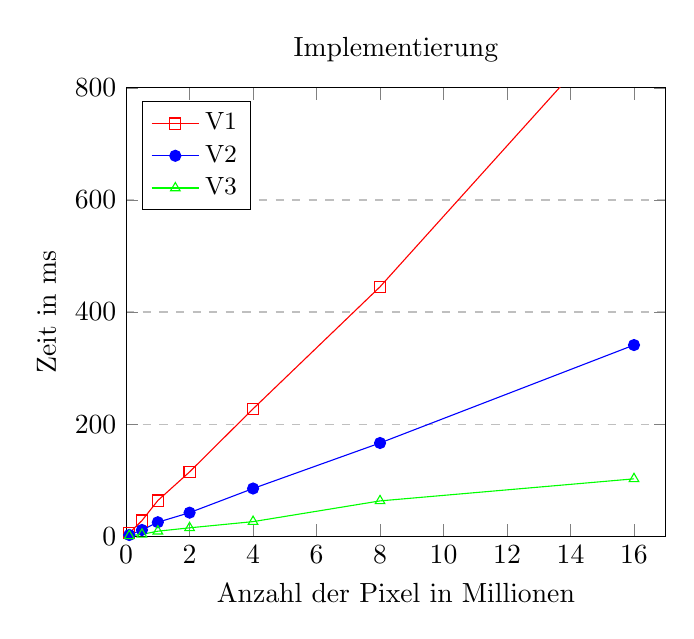
\begin{tikzpicture}
\begin{axis}[
    legend style={at={(0.5,-0.2)},anchor=north, font=\small},
    title={Implementierung},
    xlabel={Anzahl der Pixel in Millionen},
    ylabel={Zeit in ms},
    xmin=0, xmax=17,
    ymin=0, ymax=800,
    legend pos=north west,
    ymajorgrids=true,
    grid style=dashed,
]

\addplot[
    color=red,
    mark=square,
    ]
    coordinates {
    (0.1,5.5)(0.5,27.88)(1,63.66)(2,114.74)(4,227.27)(8,445.08)(16,947.94)
    };
    \addlegendentry{V1}

\addplot[
    color=blue,
    mark=*,
    ]
    coordinates {
    (0.1,2.12)(0.5,11.1)(1,24.92)(2,42.0)(4,85.10)(8,166.32)(16,341.10)
    };
    \addlegendentry{V2}

\addplot[
    color=green,
    mark=triangle,
    ]
    coordinates {
    (0.1,0.73)(0.5,3.29)(1,8.92)(2,14.94)(4,26.0)(8,62.99)(16,102.36)
    };
    \addlegendentry{V3}

\end{axis}
\end{tikzpicture}
Im ersten Diagramm, das die Laufzeit bei zunehmender Pixelanzahl darstellt, zeigen die naive und die algorithmisch optimierte Version einen ähnlichen linearen Anstieg der Zeit, was auf eine Komplexität von \( O(n) \) hindeutet, bei der die Verarbeitungszeit pro Pixel mit einer Steigung von \( 7.1 \times 10^{-5} \) ms\(\cdot\)pixel\(^{-1}\) konstant bleibt. Im Gegensatz dazu zeigt die SIMD-Implementierung eine deutlich flachere Steigung (\( 1.1 \times 10^{-5} \) ms\(\cdot\)pixel\(^{-1}\)),da Mit steigender Anzahl der Sektoren erhöht sich ebenso die Leistungsfähigkeit der SIMD. was auf eine effizientere Pixelverarbeitung schließen lässt. Mit zunehmender Pixelanzahl wird die Effizienz der SIMD deutlicher, insbesondere bei größeren Bilddaten, aufgrund ihrer Fähigkeit zur parallelen Verarbeitung.


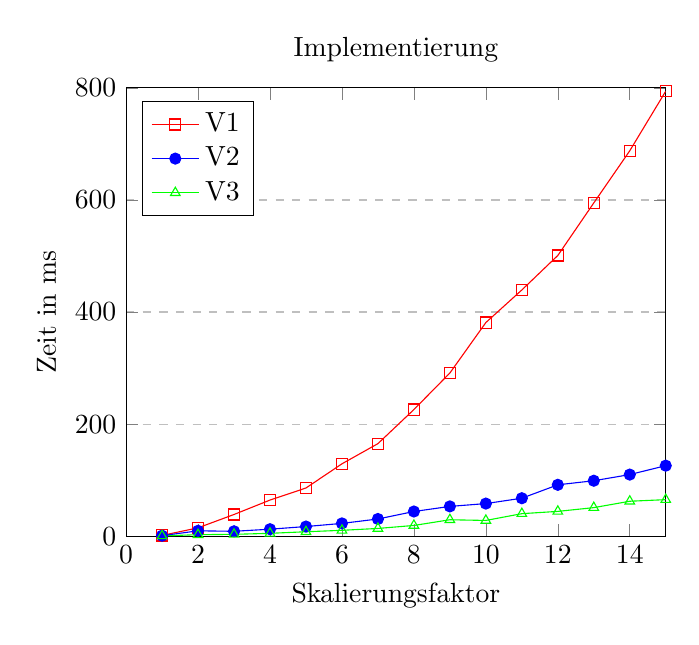
\begin{tikzpicture}
\begin{axis}[
    title={Implementierung},
    xlabel={Skalierungsfaktor},
    ylabel={Zeit in ms},
    xmin=0, xmax=15,
    ymin=0, ymax=800,
    xtick={0,2,4,6,8,10,12,14,16},
    ytick={0,200,400,600,800},
    legend pos=north west,
    ymajorgrids=true,
    grid style=dashed,
    scaled ticks=false,
    tick label style={/pgf/number format/fixed},
]

\addplot[
    color=red,
    mark=square,
    ]
    coordinates {
    (1,1.347)(2,14.953)(3,38.728)(4,64.501)(5,86.003)(6,129.159)(7,165.171)(8,226.019)(9,291.192)(10,381.240)(11,439.381)(12,500.906)(13,594.713)(14,687.771)(15,794.090)
    };
    \addlegendentry{V1}

\addplot[
    color=blue,
    mark=*,
    ]
    coordinates {
    (1,0.935)(2,9.602)(3,8.756)(4,12.495)(5,17.233)(6,22.817)(7,30.697)(8,44.067)(9,53.159)(10,58.192)(11,67.767)(12,91.688)(13,98.978)(14,109.932)(15,125.871)
    };
    \addlegendentry{V2}

\addplot[
    color=green,
    mark=triangle,
    ]
    coordinates {
    (1,0.517)(2,2.707)(3,3.307)(4,5.134)(5,7.914)(6,10.487)(7,13.839)(8,19.170)(9,29.339)(10,28.107)(11,40.195)(12,44.276)(13,50.974)(14,62.360)(15,65.233)
    };
    \addlegendentry{V3}

\end{axis}
\end{tikzpicture} \\

Das zweite Diagramm stellt die Laufzeit in Abhängigkeit von ansteigenden Skalierungsfaktoren von 1 bis 15 dar. Die naive Implementierung zeigt hierbei einen steilen, linearen Anstieg der Laufzeit mit zunehmendem Skalierungsfaktor, was auf eine direkte Korrelation zwischen Skalierungsfaktor und Zeitkomplexität hinweist.

Die beiden anderen Implementierungen hingegen weisen im Vergleich zur naiven Implementierung einen moderateren Anstieg der Laufzeit auf. Für Skalierungsfaktoren kleiner als 4 ist der Unterschied in der Leistung bemerkenswert, jedoch nicht übermäßig groß. Bei weiter ansteigenden Skalierungsfaktoren beweisen sie jedoch eine wesentlich bessere Performance. Die SIMD-Implementierung ist nach wie vor die dominierende, da sie die flachste Steigung der drei aufweist und eine relativ konstante sowie niedrige Laufzeit beibehält, was sie zur effizientesten Implementierung für die Verarbeitung in großem Maßstab macht.


\begin{table}[ht]
\centering
\begin{tabular}{|c|c|c|c|c|c|}
\hline
Pixel & V1 (ms) & V2 (ms) & V3 (ms) & V1/V3 (\%) & V1/V2. (\%) \\ 
\hline
100k & 5.5 & 2.12 & 0.73 & 753.42 & 259.62 \\
500k & 27.88 & 11.1 & 3.29 & 847.05 & 251.17 \\
1 Mil & 63.66 & 24.92 & 8.92 & 714.29 & 255.68 \\
2 Mil & 114.74 & 42.0 & 14.94 & 768.41 & 273.19 \\
4 Mil & 227.27 & 85.10 & 26.0 & 874.12 & 267.13 \\
8 Mil & 445.08 & 166.32 & 62.99 & 706.65 & 267.62 \\
16 Mil & 947.94 & 341.10 & 102.36 & 926.44 & 277.98 \\
\hline
\end{tabular}
\caption{Laufzeitgergleich der Implementationsmethoden mit Skalierungsfaktor 2}
\label{table:comparison2}
\end{table}



\subsection{Cache}
Aufgrund der Größe des resultierenden Bildes passt das Bild in keinen der L-Caches, wodurch die Speicherung vermutlich auf dem Hauptspeicher erfolgt und damit die Laufzeit des Programmes beeinträchtigt.

\section{Zusammenfassung und Ausblick}
Dieses Projekt setzt sich mit der Bildmanipulation auseinander. Dabei liegt der Fokus auf die Umwandlung von Farbbildern in Graustufen und eine anschließende Skalierung durch bilineare Interpolation. Das Programm beinhaltet neben einem naiven Ansatz zum Nachvollziehen der mathematischen Berechnungen und der theoretischen Überlegungen auch verschiedene optimierte Ansätze, die je nach Kontext und Einbettung des Programms bessere Resultate liefern. Hierbei kommen algorithmische Optimierungen wie Look-up-Tables, die vorab Werte berechnen, sowie Parallelisierung durch SIMD zum Einsatz, um eine maximale Leistungsfähigkeit des Codes zu gewährleisten.\\\\
Dieses Projekt ist nicht nur theoretisch von besonderer Bedeutung, auch praktisch finden sich Graustufenkonvertierung und bilineare Interpolation viele sinnvolle Anwendungsmöglichkeiten. So wird die Graustufenkonvertierung oft in der Bild- und Videoverarbeitung verwendet, um Retro-Effekte nachzuahmen oder um Speicher zu sparen, wenn die Farbinformationen keine Rolle spielen. Die Integration der bilinearen Interpolation macht den Algorithmus auch bedeutsam für Videokompression und Computerspiele. So lässt sich ein Bild zuerst komprimieren und dann interpolieren, um Speicher zu sparen.\\
Dieses Projekt demonstriert, wie mathematischen Erkenntnisse und technische Grundlagen innovative Bildverarbeitungstechniken hervorbringen können, die die Bildqualität und die Bildrepräsentation revolutionieren können. Insgesamt kann das Projekt als Grundlage für viele weitere Arbeiten im Bereich der Bildmanipulation dienen.

% TODO: Fuegen Sie Ihre Quellen der Datei Ausarbeitung.bib hinzu
% Referenzieren Sie diese dann mit \cite{}.
% Beispiel: CR2 ist ein Register der x86-Architektur~\cite{intel2017man}.
\bibliographystyle{plain}
\bibliography{Ausarbeitung}{

\cite{ece472}
\cite{ppm}
\cite{ppmformats}
\cite{pgmpgmpbm}
\cite{grafikgraustufen}
\cite{bilint}
\cite{wahrnehmung}

}

\end{document}